% Options for packages loaded elsewhere
\PassOptionsToPackage{unicode}{hyperref}
\PassOptionsToPackage{hyphens}{url}
\PassOptionsToPackage{dvipsnames,svgnames,x11names}{xcolor}
%
\documentclass[
  letterpaper,
  DIV=11,
  numbers=noendperiod]{scrartcl}

\usepackage{amsmath,amssymb}
\usepackage{iftex}
\ifPDFTeX
  \usepackage[T1]{fontenc}
  \usepackage[utf8]{inputenc}
  \usepackage{textcomp} % provide euro and other symbols
\else % if luatex or xetex
  \usepackage{unicode-math}
  \defaultfontfeatures{Scale=MatchLowercase}
  \defaultfontfeatures[\rmfamily]{Ligatures=TeX,Scale=1}
\fi
\usepackage{lmodern}
\ifPDFTeX\else  
    % xetex/luatex font selection
\fi
% Use upquote if available, for straight quotes in verbatim environments
\IfFileExists{upquote.sty}{\usepackage{upquote}}{}
\IfFileExists{microtype.sty}{% use microtype if available
  \usepackage[]{microtype}
  \UseMicrotypeSet[protrusion]{basicmath} % disable protrusion for tt fonts
}{}
\makeatletter
\@ifundefined{KOMAClassName}{% if non-KOMA class
  \IfFileExists{parskip.sty}{%
    \usepackage{parskip}
  }{% else
    \setlength{\parindent}{0pt}
    \setlength{\parskip}{6pt plus 2pt minus 1pt}}
}{% if KOMA class
  \KOMAoptions{parskip=half}}
\makeatother
\usepackage{xcolor}
\setlength{\emergencystretch}{3em} % prevent overfull lines
\setcounter{secnumdepth}{-\maxdimen} % remove section numbering
% Make \paragraph and \subparagraph free-standing
\ifx\paragraph\undefined\else
  \let\oldparagraph\paragraph
  \renewcommand{\paragraph}[1]{\oldparagraph{#1}\mbox{}}
\fi
\ifx\subparagraph\undefined\else
  \let\oldsubparagraph\subparagraph
  \renewcommand{\subparagraph}[1]{\oldsubparagraph{#1}\mbox{}}
\fi

\usepackage{color}
\usepackage{fancyvrb}
\newcommand{\VerbBar}{|}
\newcommand{\VERB}{\Verb[commandchars=\\\{\}]}
\DefineVerbatimEnvironment{Highlighting}{Verbatim}{commandchars=\\\{\}}
% Add ',fontsize=\small' for more characters per line
\usepackage{framed}
\definecolor{shadecolor}{RGB}{241,243,245}
\newenvironment{Shaded}{\begin{snugshade}}{\end{snugshade}}
\newcommand{\AlertTok}[1]{\textcolor[rgb]{0.68,0.00,0.00}{#1}}
\newcommand{\AnnotationTok}[1]{\textcolor[rgb]{0.37,0.37,0.37}{#1}}
\newcommand{\AttributeTok}[1]{\textcolor[rgb]{0.40,0.45,0.13}{#1}}
\newcommand{\BaseNTok}[1]{\textcolor[rgb]{0.68,0.00,0.00}{#1}}
\newcommand{\BuiltInTok}[1]{\textcolor[rgb]{0.00,0.23,0.31}{#1}}
\newcommand{\CharTok}[1]{\textcolor[rgb]{0.13,0.47,0.30}{#1}}
\newcommand{\CommentTok}[1]{\textcolor[rgb]{0.37,0.37,0.37}{#1}}
\newcommand{\CommentVarTok}[1]{\textcolor[rgb]{0.37,0.37,0.37}{\textit{#1}}}
\newcommand{\ConstantTok}[1]{\textcolor[rgb]{0.56,0.35,0.01}{#1}}
\newcommand{\ControlFlowTok}[1]{\textcolor[rgb]{0.00,0.23,0.31}{#1}}
\newcommand{\DataTypeTok}[1]{\textcolor[rgb]{0.68,0.00,0.00}{#1}}
\newcommand{\DecValTok}[1]{\textcolor[rgb]{0.68,0.00,0.00}{#1}}
\newcommand{\DocumentationTok}[1]{\textcolor[rgb]{0.37,0.37,0.37}{\textit{#1}}}
\newcommand{\ErrorTok}[1]{\textcolor[rgb]{0.68,0.00,0.00}{#1}}
\newcommand{\ExtensionTok}[1]{\textcolor[rgb]{0.00,0.23,0.31}{#1}}
\newcommand{\FloatTok}[1]{\textcolor[rgb]{0.68,0.00,0.00}{#1}}
\newcommand{\FunctionTok}[1]{\textcolor[rgb]{0.28,0.35,0.67}{#1}}
\newcommand{\ImportTok}[1]{\textcolor[rgb]{0.00,0.46,0.62}{#1}}
\newcommand{\InformationTok}[1]{\textcolor[rgb]{0.37,0.37,0.37}{#1}}
\newcommand{\KeywordTok}[1]{\textcolor[rgb]{0.00,0.23,0.31}{#1}}
\newcommand{\NormalTok}[1]{\textcolor[rgb]{0.00,0.23,0.31}{#1}}
\newcommand{\OperatorTok}[1]{\textcolor[rgb]{0.37,0.37,0.37}{#1}}
\newcommand{\OtherTok}[1]{\textcolor[rgb]{0.00,0.23,0.31}{#1}}
\newcommand{\PreprocessorTok}[1]{\textcolor[rgb]{0.68,0.00,0.00}{#1}}
\newcommand{\RegionMarkerTok}[1]{\textcolor[rgb]{0.00,0.23,0.31}{#1}}
\newcommand{\SpecialCharTok}[1]{\textcolor[rgb]{0.37,0.37,0.37}{#1}}
\newcommand{\SpecialStringTok}[1]{\textcolor[rgb]{0.13,0.47,0.30}{#1}}
\newcommand{\StringTok}[1]{\textcolor[rgb]{0.13,0.47,0.30}{#1}}
\newcommand{\VariableTok}[1]{\textcolor[rgb]{0.07,0.07,0.07}{#1}}
\newcommand{\VerbatimStringTok}[1]{\textcolor[rgb]{0.13,0.47,0.30}{#1}}
\newcommand{\WarningTok}[1]{\textcolor[rgb]{0.37,0.37,0.37}{\textit{#1}}}

\providecommand{\tightlist}{%
  \setlength{\itemsep}{0pt}\setlength{\parskip}{0pt}}\usepackage{longtable,booktabs,array}
\usepackage{calc} % for calculating minipage widths
% Correct order of tables after \paragraph or \subparagraph
\usepackage{etoolbox}
\makeatletter
\patchcmd\longtable{\par}{\if@noskipsec\mbox{}\fi\par}{}{}
\makeatother
% Allow footnotes in longtable head/foot
\IfFileExists{footnotehyper.sty}{\usepackage{footnotehyper}}{\usepackage{footnote}}
\makesavenoteenv{longtable}
\usepackage{graphicx}
\makeatletter
\def\maxwidth{\ifdim\Gin@nat@width>\linewidth\linewidth\else\Gin@nat@width\fi}
\def\maxheight{\ifdim\Gin@nat@height>\textheight\textheight\else\Gin@nat@height\fi}
\makeatother
% Scale images if necessary, so that they will not overflow the page
% margins by default, and it is still possible to overwrite the defaults
% using explicit options in \includegraphics[width, height, ...]{}
\setkeys{Gin}{width=\maxwidth,height=\maxheight,keepaspectratio}
% Set default figure placement to htbp
\makeatletter
\def\fps@figure{htbp}
\makeatother

\KOMAoption{captions}{tableheading}
\makeatletter
\makeatother
\makeatletter
\makeatother
\makeatletter
\@ifpackageloaded{caption}{}{\usepackage{caption}}
\AtBeginDocument{%
\ifdefined\contentsname
  \renewcommand*\contentsname{Table of contents}
\else
  \newcommand\contentsname{Table of contents}
\fi
\ifdefined\listfigurename
  \renewcommand*\listfigurename{List of Figures}
\else
  \newcommand\listfigurename{List of Figures}
\fi
\ifdefined\listtablename
  \renewcommand*\listtablename{List of Tables}
\else
  \newcommand\listtablename{List of Tables}
\fi
\ifdefined\figurename
  \renewcommand*\figurename{Figure}
\else
  \newcommand\figurename{Figure}
\fi
\ifdefined\tablename
  \renewcommand*\tablename{Table}
\else
  \newcommand\tablename{Table}
\fi
}
\@ifpackageloaded{float}{}{\usepackage{float}}
\floatstyle{ruled}
\@ifundefined{c@chapter}{\newfloat{codelisting}{h}{lop}}{\newfloat{codelisting}{h}{lop}[chapter]}
\floatname{codelisting}{Listing}
\newcommand*\listoflistings{\listof{codelisting}{List of Listings}}
\makeatother
\makeatletter
\@ifpackageloaded{caption}{}{\usepackage{caption}}
\@ifpackageloaded{subcaption}{}{\usepackage{subcaption}}
\makeatother
\makeatletter
\@ifpackageloaded{tcolorbox}{}{\usepackage[skins,breakable]{tcolorbox}}
\makeatother
\makeatletter
\@ifundefined{shadecolor}{\definecolor{shadecolor}{rgb}{.97, .97, .97}}
\makeatother
\makeatletter
\makeatother
\makeatletter
\makeatother
\ifLuaTeX
  \usepackage{selnolig}  % disable illegal ligatures
\fi
\IfFileExists{bookmark.sty}{\usepackage{bookmark}}{\usepackage{hyperref}}
\IfFileExists{xurl.sty}{\usepackage{xurl}}{} % add URL line breaks if available
\urlstyle{same} % disable monospaced font for URLs
\hypersetup{
  pdftitle={Environmental Data Analysis and Visualization},
  pdfauthor={Week 1 Lecture 2},
  colorlinks=true,
  linkcolor={blue},
  filecolor={Maroon},
  citecolor={Blue},
  urlcolor={Blue},
  pdfcreator={LaTeX via pandoc}}

\title{Environmental Data Analysis and Visualization}
\author{Week 1 Lecture 2}
\date{}

\begin{document}
\maketitle
\ifdefined\Shaded\renewenvironment{Shaded}{\begin{tcolorbox}[enhanced, sharp corners, interior hidden, borderline west={3pt}{0pt}{shadecolor}, frame hidden, boxrule=0pt, breakable]}{\end{tcolorbox}}\fi

\hypertarget{sensor-of-the-day}{%
\subsection{Sensor of the day}\label{sensor-of-the-day}}

\begin{figure}

{\centering 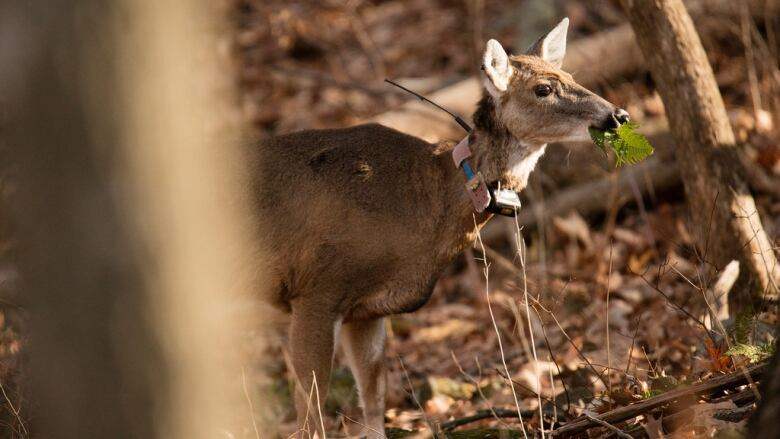
\includegraphics{InClassStatic/deer-collar.jpg}

}

\caption{(Photo credit: Shenandoah National Park via
\href{https://www.cbc.ca/news/canada/british-columbia/problem-deer-get-gps-collars-ahead-of-oak-bay-birth-control-plan-1.4031937}{CBC.ca})}

\end{figure}

\hypertarget{sensor-of-the-day-1}{%
\subsection{Sensor of the day}\label{sensor-of-the-day-1}}

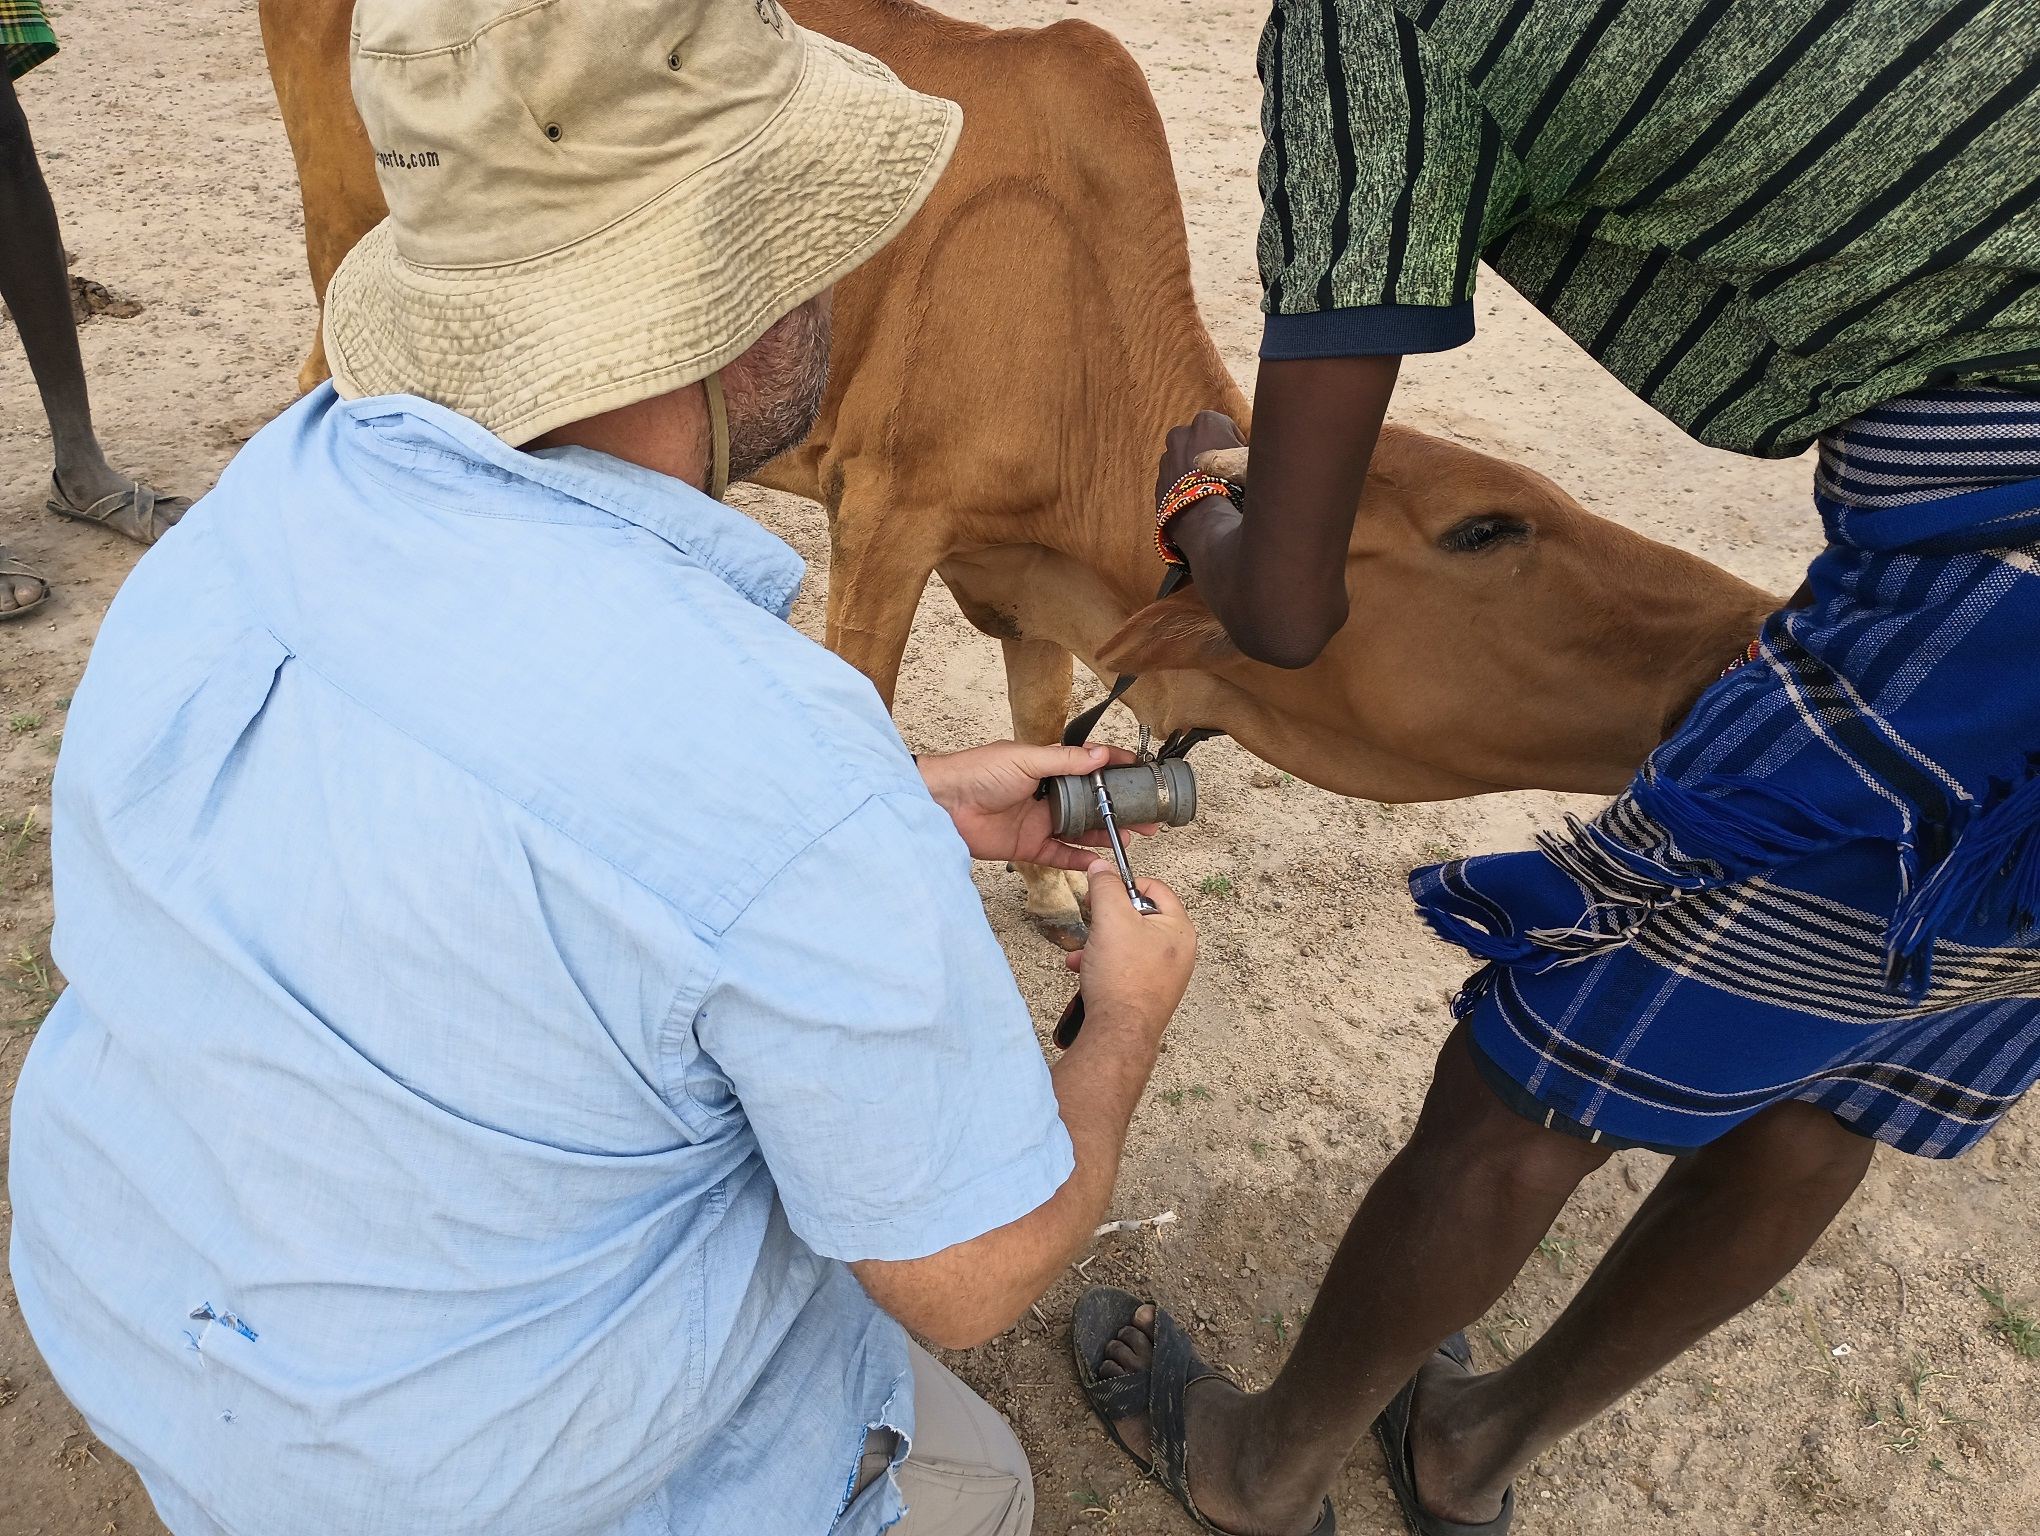
\includegraphics{InClassStatic/gpsCollar.jpg}

\hypertarget{sensor-of-the-day-2}{%
\subsection{Sensor of the day}\label{sensor-of-the-day-2}}

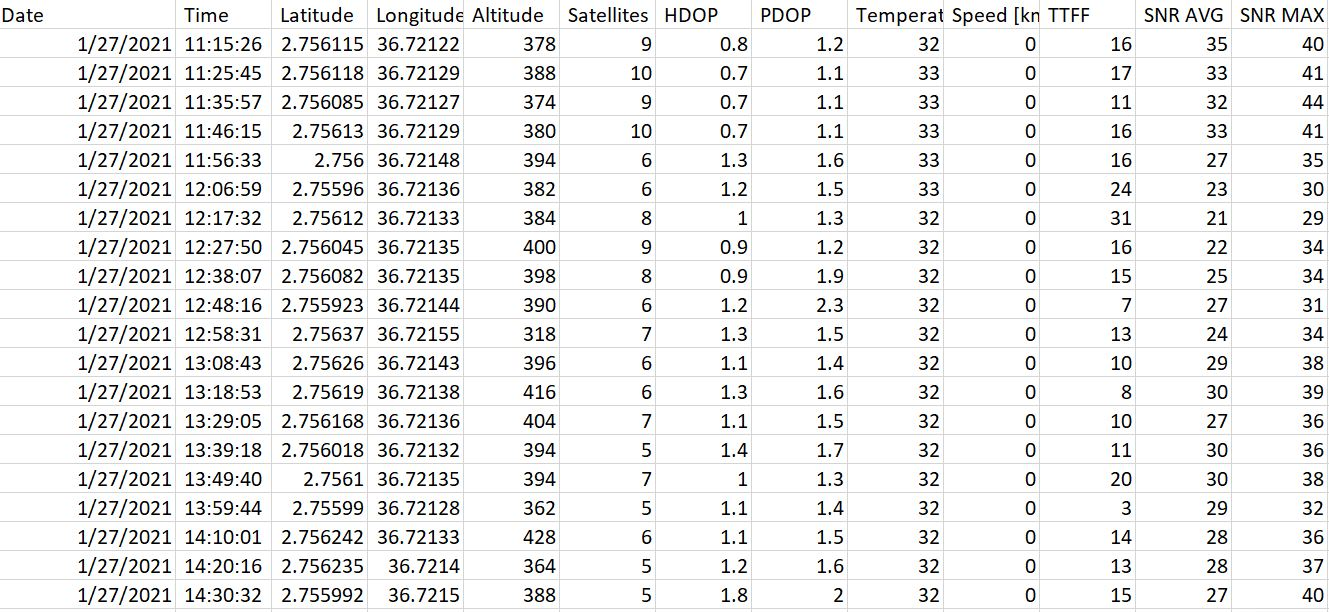
\includegraphics{InClassStatic/collarData.JPG}

\hypertarget{sensor-of-the-day-3}{%
\subsection{Sensor of the day}\label{sensor-of-the-day-3}}

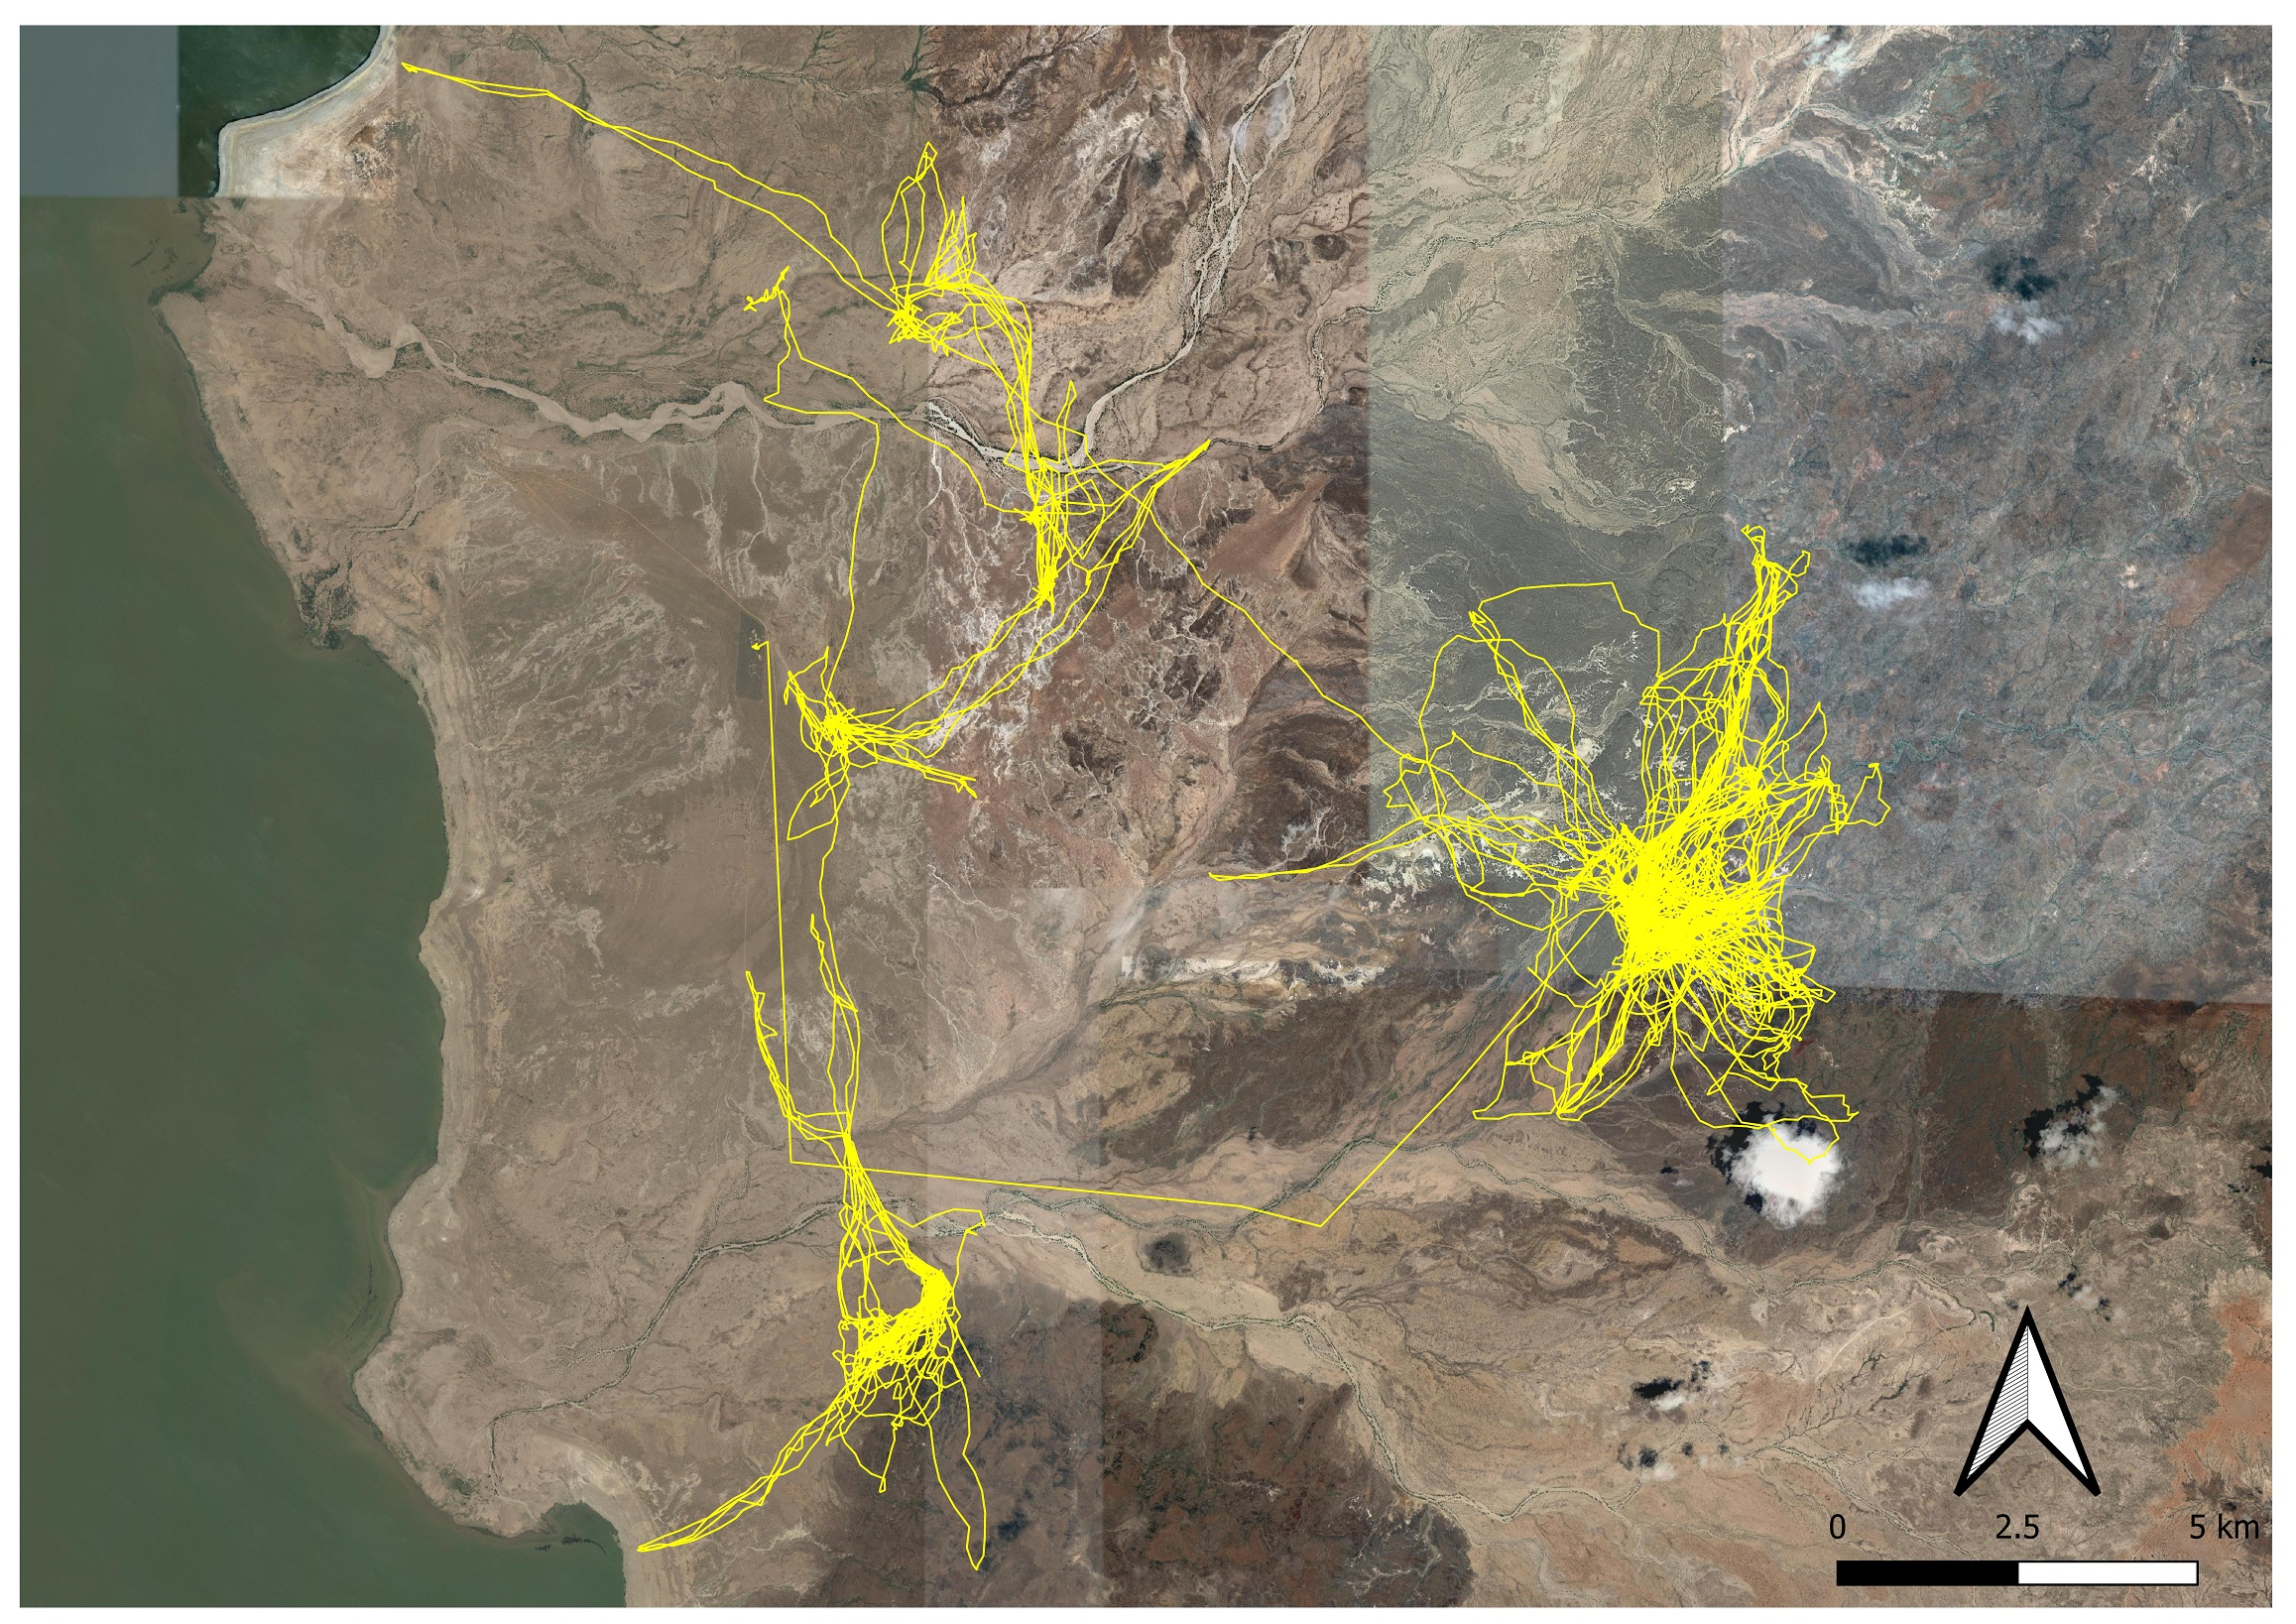
\includegraphics{InClassStatic/animaltracks.jpg}

\hypertarget{sensor-of-the-day-4}{%
\subsection{Sensor of the day}\label{sensor-of-the-day-4}}

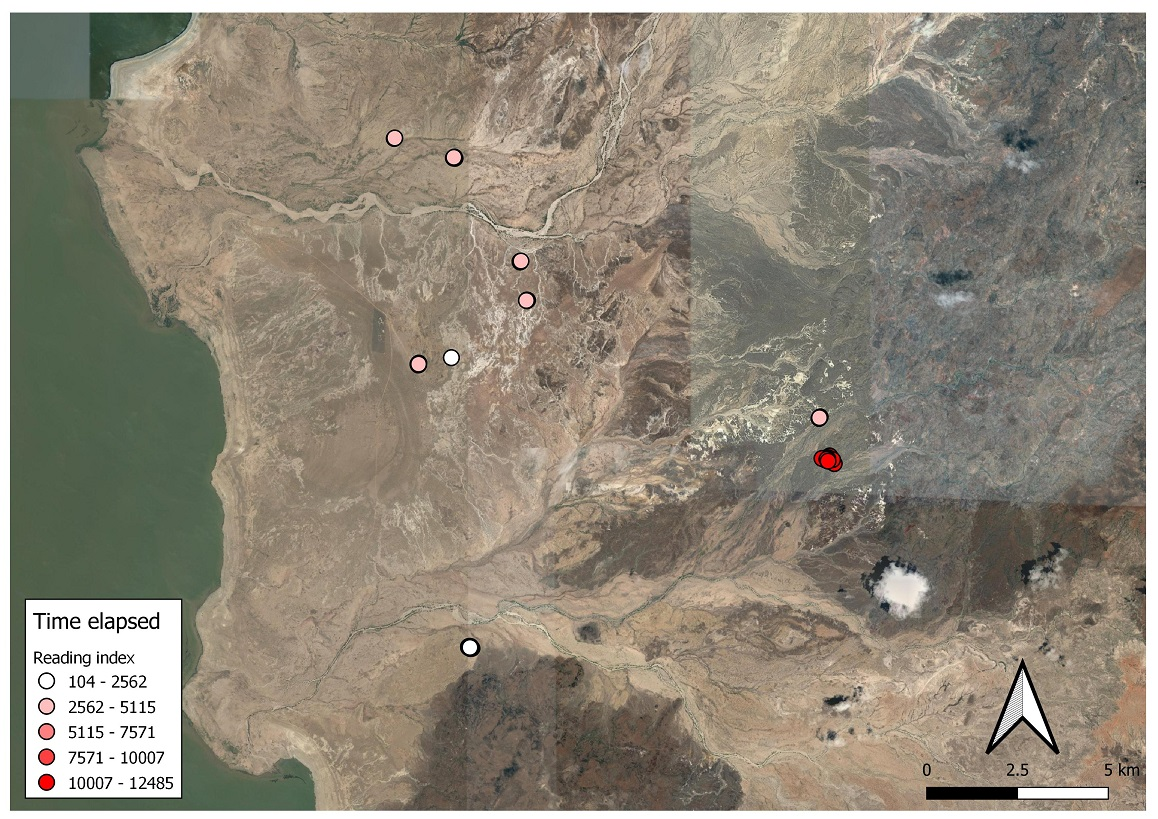
\includegraphics{InClassStatic/camps.jpg}

\hypertarget{movebank}{%
\subsection{Movebank}\label{movebank}}

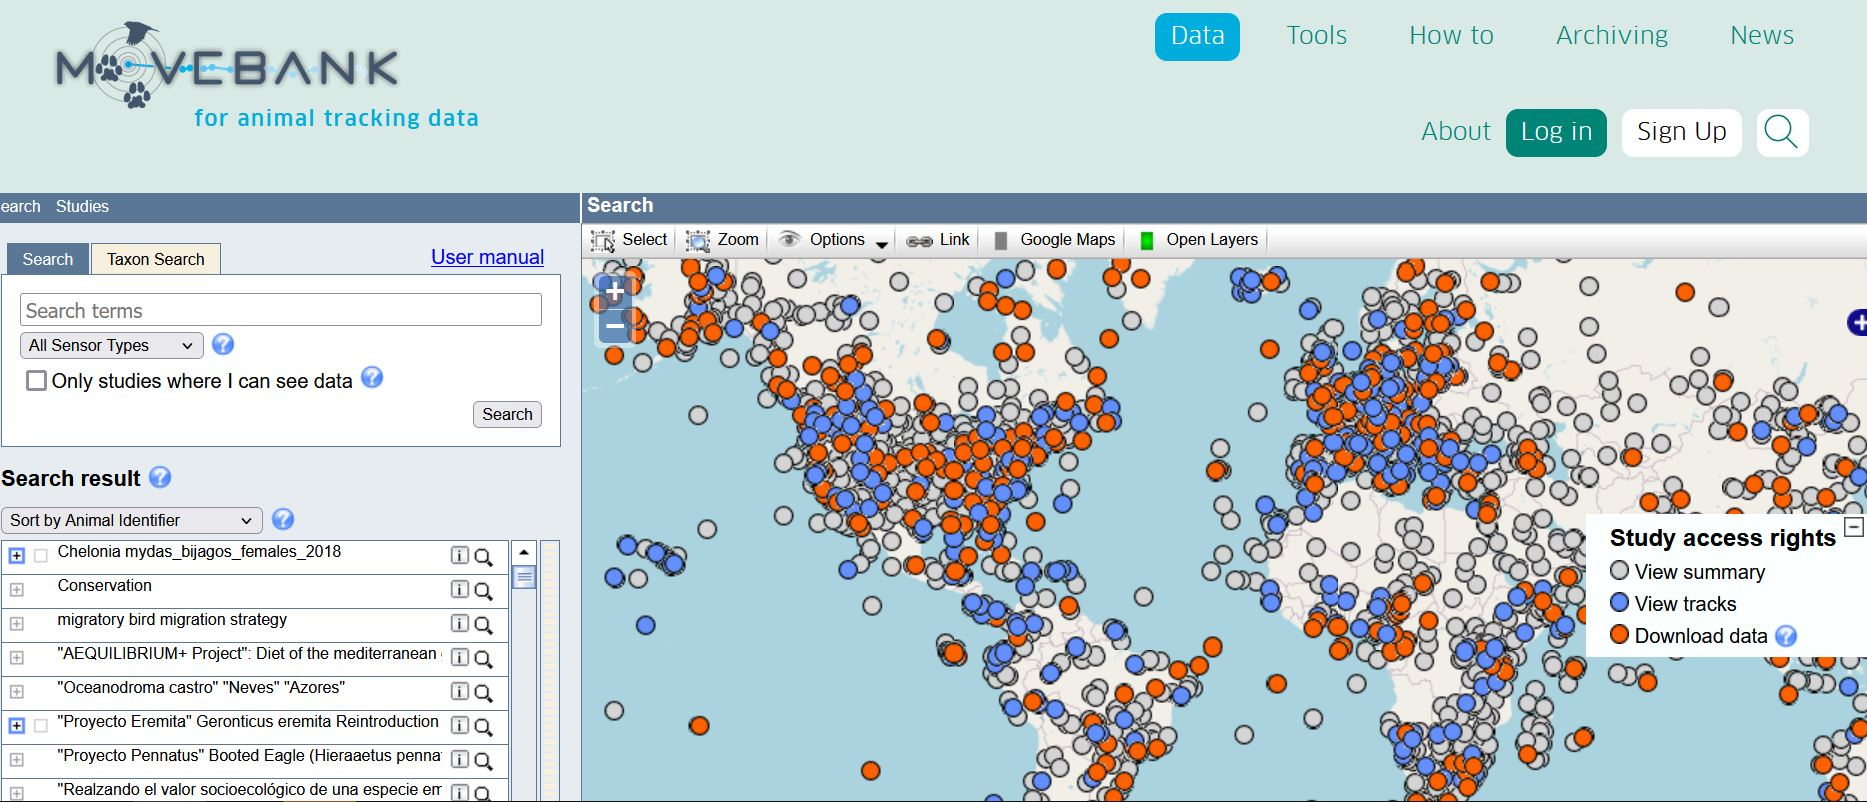
\includegraphics{InClassStatic/movebank.JPG}

\url{https://www.movebank.org/}

\hypertarget{about-this-course}{%
\subsection{About this course}\label{about-this-course}}

This course is designed to develop skills and knowledge needed to
assemble, manage, visualize, analyze, and communicate about
environmental data. Students will learn fundamental data science
concepts and computational techniques needed to

\begin{itemize}
\item
  access data from a variety of sources;
\item
  organize and reshape datasets to suit different purposes;
\item
  plot data to evaluate patterns;
\item
  assess the robustness and uniqueness of those patterns;
\item
  share their findings to different audiences.
\end{itemize}

\hypertarget{section}{%
\subsection{}\label{section}}

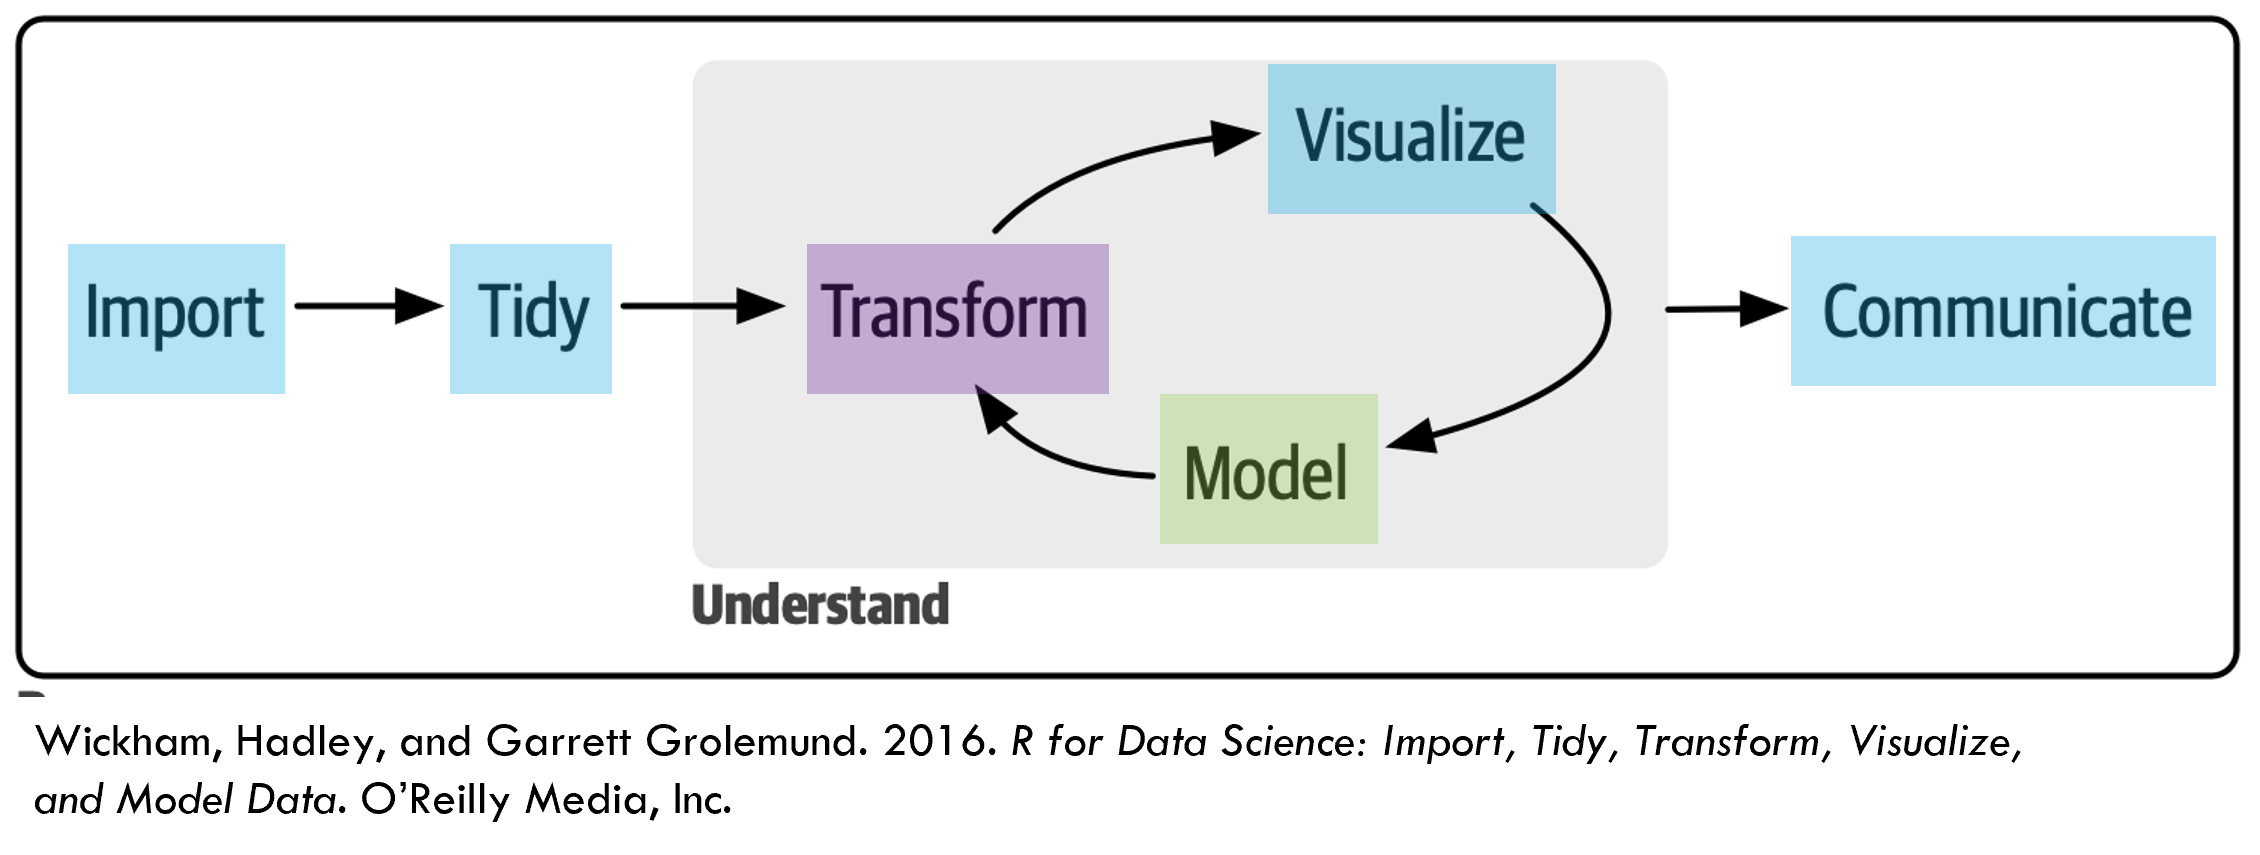
\includegraphics{InClassStatic/dataSciencePipeline.png}

\hypertarget{about-this-course-1}{%
\subsection{About this course}\label{about-this-course-1}}

Students will also explore how aesthetic design choices contribute to
the usefulness of visualizations for telling environmental stories and
best practices for making data and open and accessible for public reuse.

\hypertarget{why-use-data-to-build-narratives}{%
\subsection{Why use data to build
narratives?}\label{why-use-data-to-build-narratives}}

\url{https://www.youtube.com/watch?v=ph439t-kTIE}

\hypertarget{section-1}{%
\subsection{}\label{section-1}}

\url{https://svs.gsfc.nasa.gov/vis/a000000/a005100/a005137/GISTEMP_Curves_July2023_1080p60.mp4}
NASA Scientific Visualization Studio (https://svs.gsfc.nasa.gov/5137/)

\hypertarget{section-2}{%
\subsection{}\label{section-2}}

\begin{figure}

{\centering 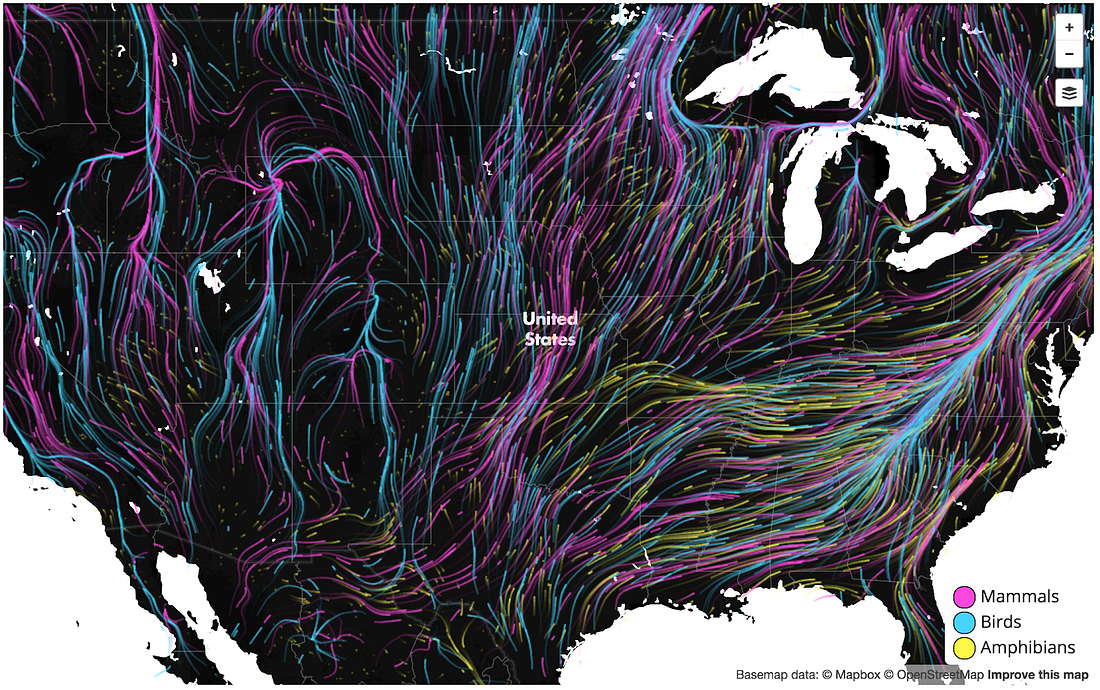
\includegraphics{InClassStatic/migrations.png}

}

\caption{Nature Conservancy
(http://maps.tnc.org/migrations-in-motion/\#5/38.376/-104.985)}

\end{figure}

\hypertarget{section-3}{%
\subsection{}\label{section-3}}

\begin{figure}

{\centering 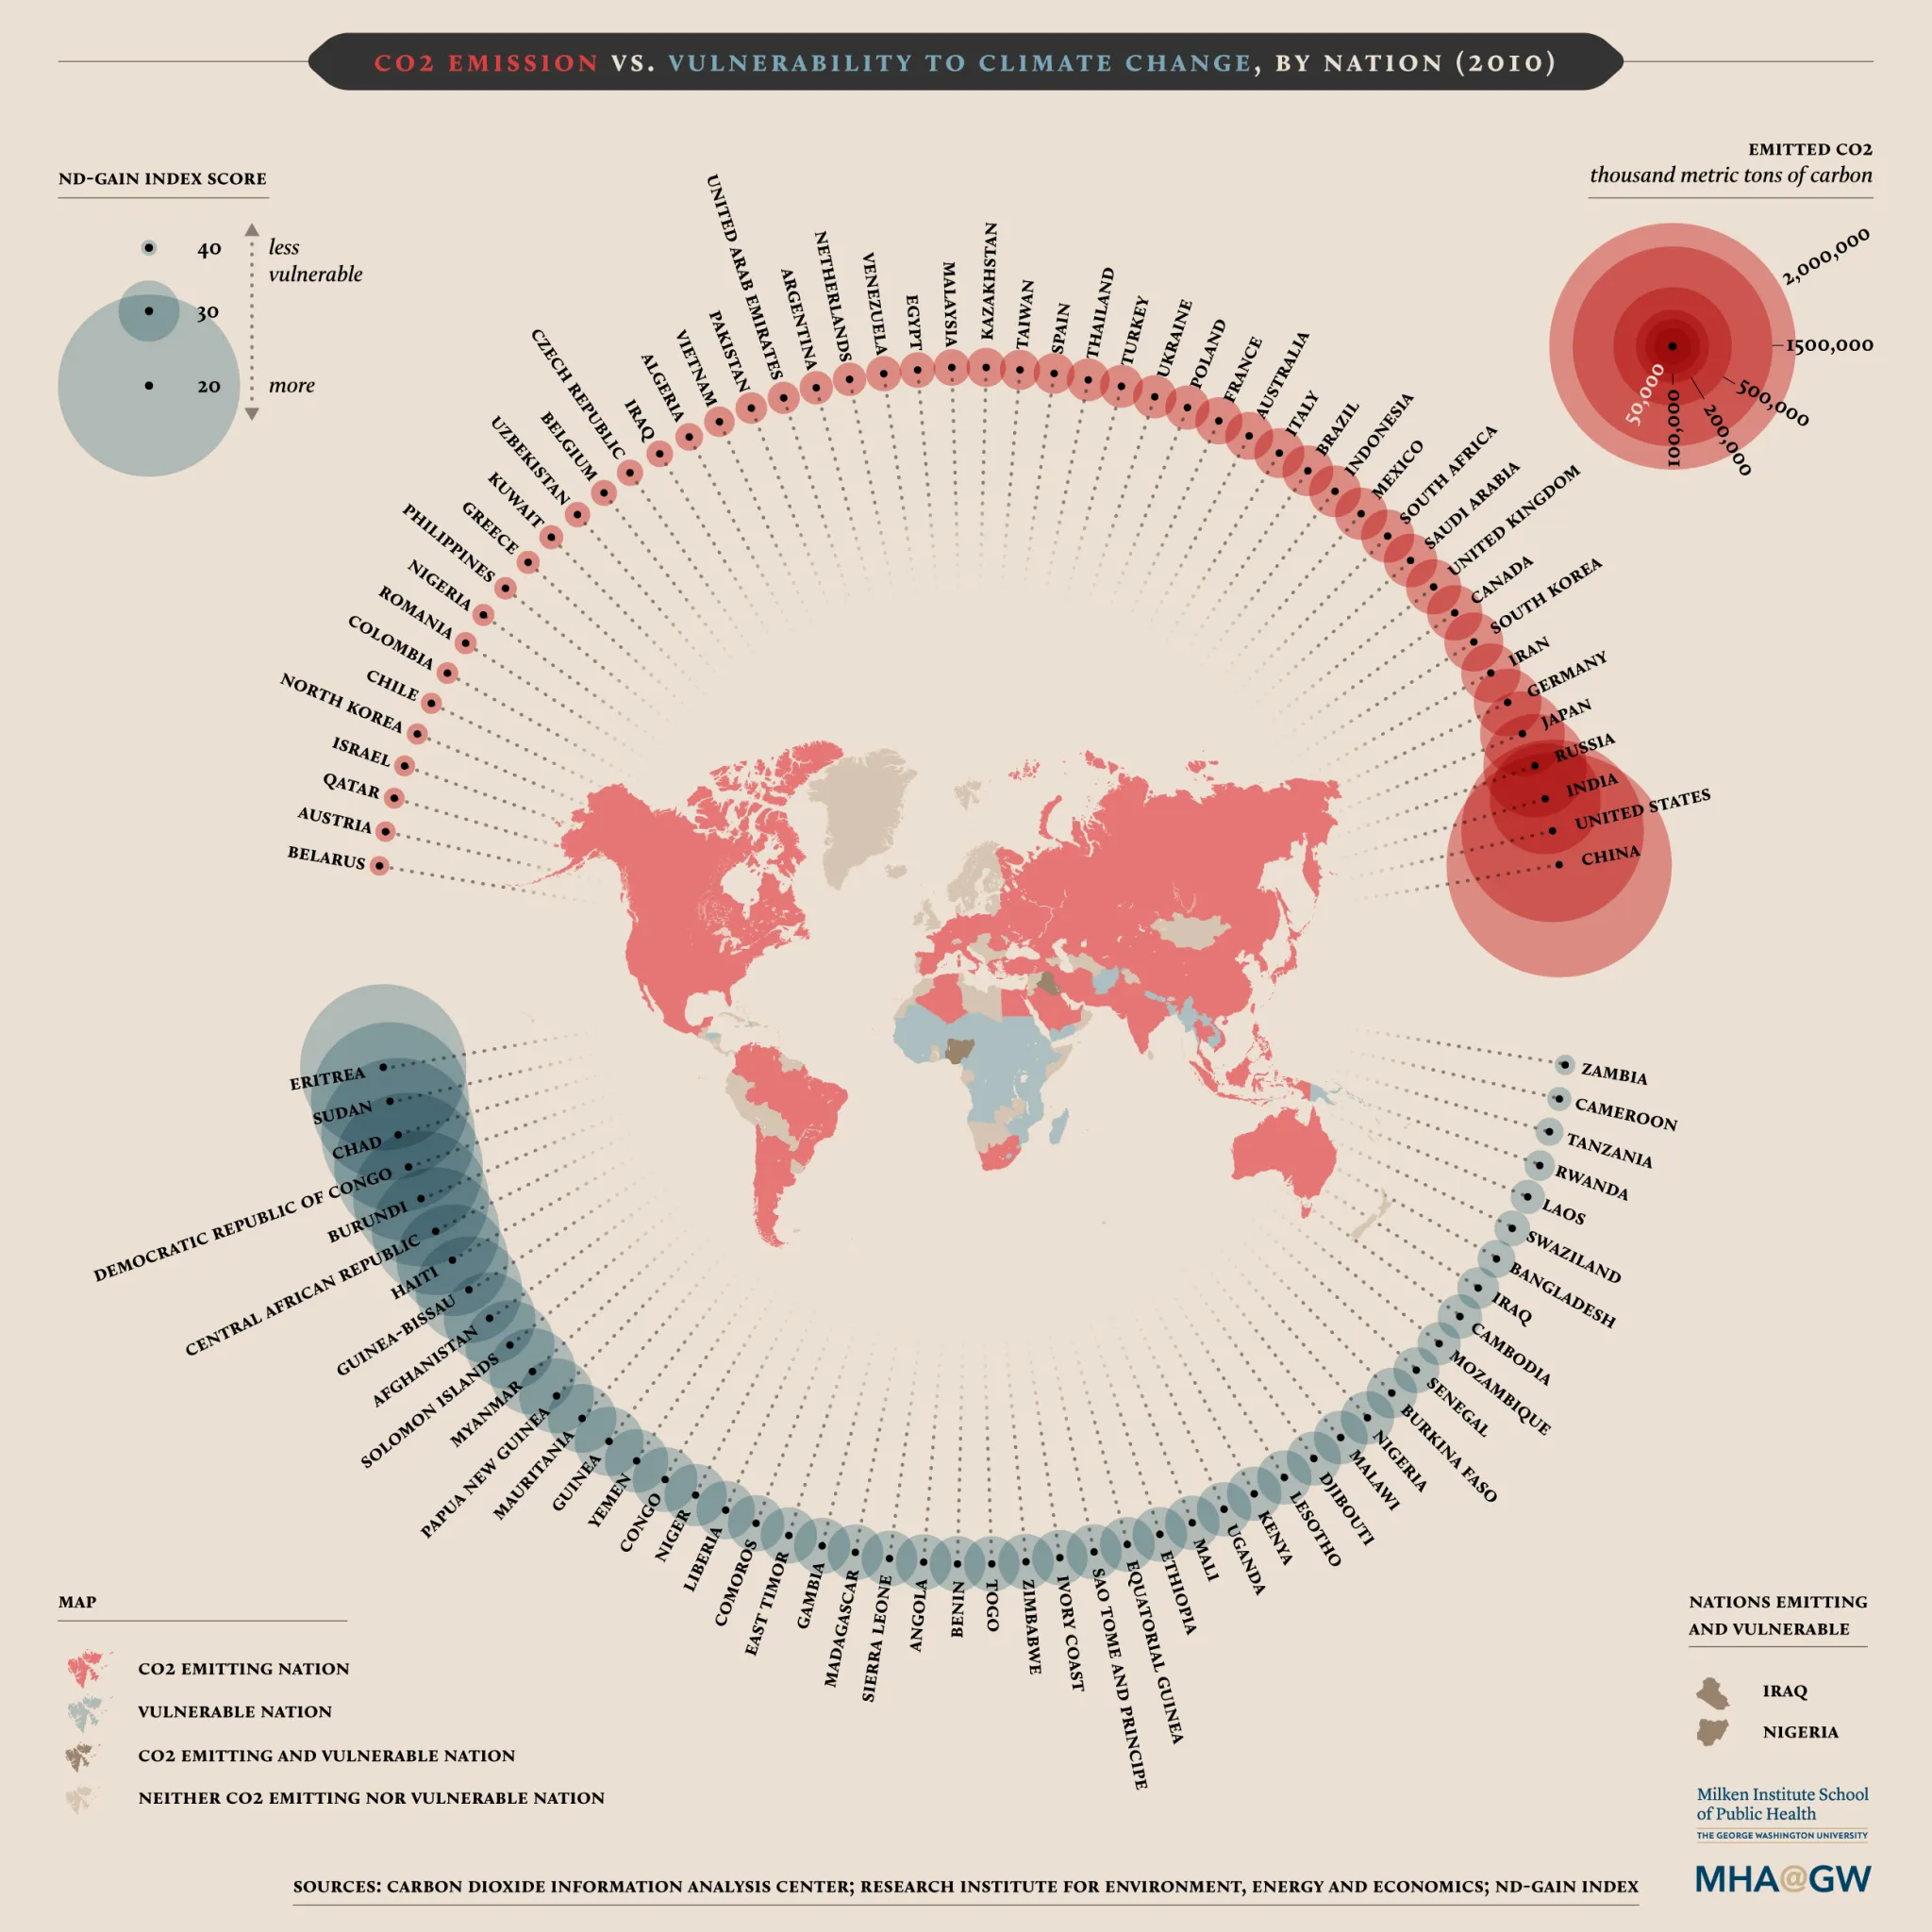
\includegraphics{InClassStatic/Climate_Change_carbon_v_vulnerability.png}

}

\caption{\href{http://publichealth.gwu.edu/}{Milken Institute School of
Public Health}~at the George Washington University
(\url{https://onlinepublichealth.gwu.edu/resources/climate-change-emissions-data/})}

\end{figure}

\hypertarget{section-4}{%
\subsection{}\label{section-4}}

\begin{figure}

{\centering 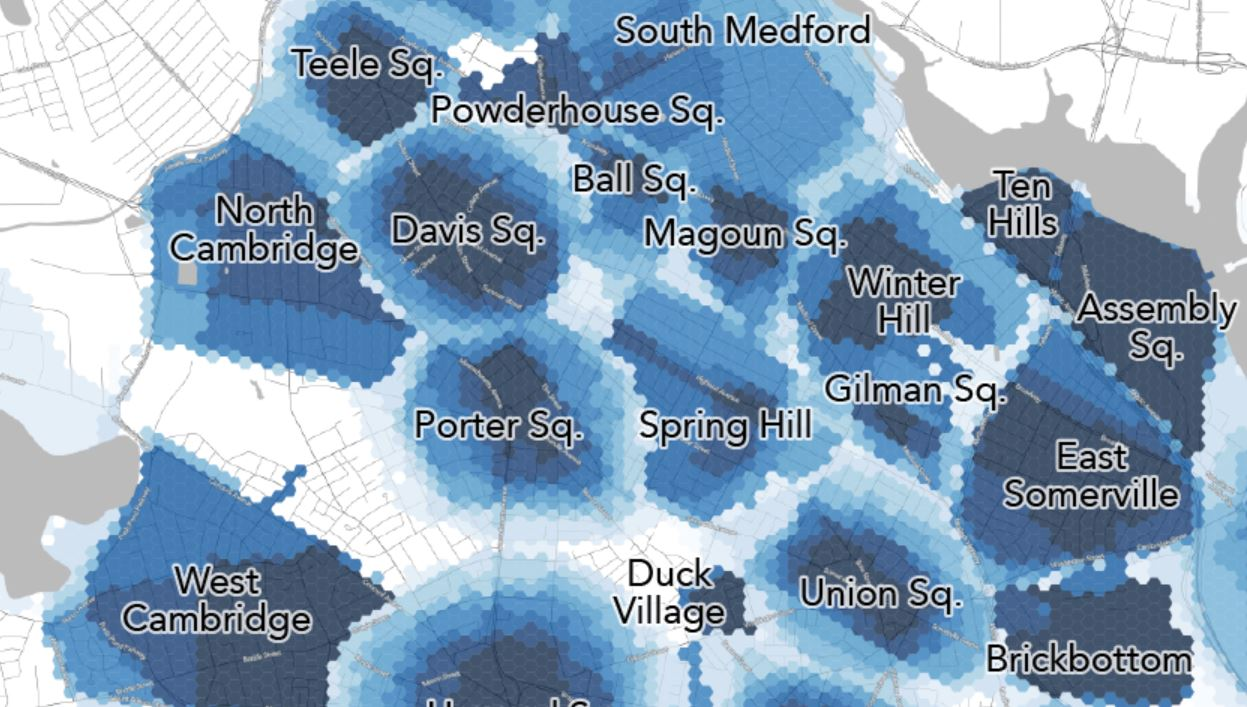
\includegraphics{InClassStatic/BostonNeighborhoods.JPG}

}

\caption{Crowdsourced neighborhood boundaries
(https://bostonography.com/2017/official-unofficial-neighborhoods-2017/)}

\end{figure}

\hypertarget{how-we-get-there}{%
\subsection{How we get there}\label{how-we-get-there}}


\includegraphics[width=4.07292in,height=\textheight]{InClassStatic/rLogo.png}


\includegraphics{InClassStatic/RStudio-Logo-Flat.png}

\hypertarget{how-we-get-there-1}{%
\subsection{How we get there}\label{how-we-get-there-1}}

\begin{Shaded}
\begin{Highlighting}[]
\FunctionTok{library}\NormalTok{(ggplot2)}


\NormalTok{sepal.labels }\OtherTok{\textless{}{-}} \FunctionTok{labs}\NormalTok{(}\AttributeTok{x =} \StringTok{"Sepal Length (cm)"}\NormalTok{, }\AttributeTok{y =} \StringTok{"Sepal Width (cm)"}\NormalTok{,}
                     \AttributeTok{title =} \StringTok{"Relationship between Sepal Length and Width"}\NormalTok{,}
                     \AttributeTok{caption =} \StringTok{"data from Anderson (1935)"}\NormalTok{)}
\NormalTok{my.theme }\OtherTok{\textless{}{-}} \FunctionTok{theme\_classic}\NormalTok{()  }\SpecialCharTok{+} \FunctionTok{theme}\NormalTok{(}\AttributeTok{aspect.ratio =} \DecValTok{1}\NormalTok{)}

\NormalTok{all.sepals }\OtherTok{\textless{}{-}} \FunctionTok{ggplot}\NormalTok{(iris, }\FunctionTok{aes}\NormalTok{(}\AttributeTok{x =}\NormalTok{ Sepal.Length, }\AttributeTok{y =}\NormalTok{ Sepal.Width))}

\NormalTok{all.sepals }\SpecialCharTok{+} 
  \FunctionTok{geom\_point}\NormalTok{(}\FunctionTok{aes}\NormalTok{(}\AttributeTok{color =}\NormalTok{ Species, }\AttributeTok{shape =}\NormalTok{ Species), }\AttributeTok{size =} \DecValTok{2}\NormalTok{, }\AttributeTok{alpha =} \FloatTok{0.6}\NormalTok{) }\SpecialCharTok{+}
\NormalTok{  sepal.labels }\SpecialCharTok{+} \FunctionTok{labs}\NormalTok{(}\AttributeTok{subtitle =} \StringTok{"All species"}\NormalTok{) }\SpecialCharTok{+}
\NormalTok{  my.theme}
\end{Highlighting}
\end{Shaded}

\hypertarget{how-we-get-there-2}{%
\subsection{How we get there}\label{how-we-get-there-2}}

\begin{Shaded}
\begin{Highlighting}[]
\FunctionTok{library}\NormalTok{(ggplot2)}


\NormalTok{sepal.labels }\OtherTok{\textless{}{-}} \FunctionTok{labs}\NormalTok{(}\AttributeTok{x =} \StringTok{"Sepal Length (cm)"}\NormalTok{, }\AttributeTok{y =} \StringTok{"Sepal Width (cm)"}\NormalTok{,}
                     \AttributeTok{title =} \StringTok{"Relationship between Sepal Length and Width"}\NormalTok{,}
                     \AttributeTok{caption =} \StringTok{"data from Anderson (1935)"}\NormalTok{)}
\NormalTok{my.theme }\OtherTok{\textless{}{-}} \FunctionTok{theme\_classic}\NormalTok{()  }\SpecialCharTok{+} \FunctionTok{theme}\NormalTok{(}\AttributeTok{aspect.ratio =} \DecValTok{1}\NormalTok{)}

\NormalTok{all.sepals }\OtherTok{\textless{}{-}} \FunctionTok{ggplot}\NormalTok{(iris, }\FunctionTok{aes}\NormalTok{(}\AttributeTok{x =}\NormalTok{ Sepal.Length, }\AttributeTok{y =}\NormalTok{ Sepal.Width))}

\NormalTok{all.sepals }\SpecialCharTok{+} 
  \FunctionTok{geom\_point}\NormalTok{(}\FunctionTok{aes}\NormalTok{(}\AttributeTok{color =}\NormalTok{ Species, }\AttributeTok{shape =}\NormalTok{ Species), }\AttributeTok{size =} \DecValTok{2}\NormalTok{, }\AttributeTok{alpha =} \FloatTok{0.6}\NormalTok{) }\SpecialCharTok{+}
\NormalTok{  sepal.labels }\SpecialCharTok{+} \FunctionTok{labs}\NormalTok{(}\AttributeTok{subtitle =} \StringTok{"All species"}\NormalTok{) }\SpecialCharTok{+}
\NormalTok{  my.theme}
\end{Highlighting}
\end{Shaded}

\begin{figure}[H]

{\centering 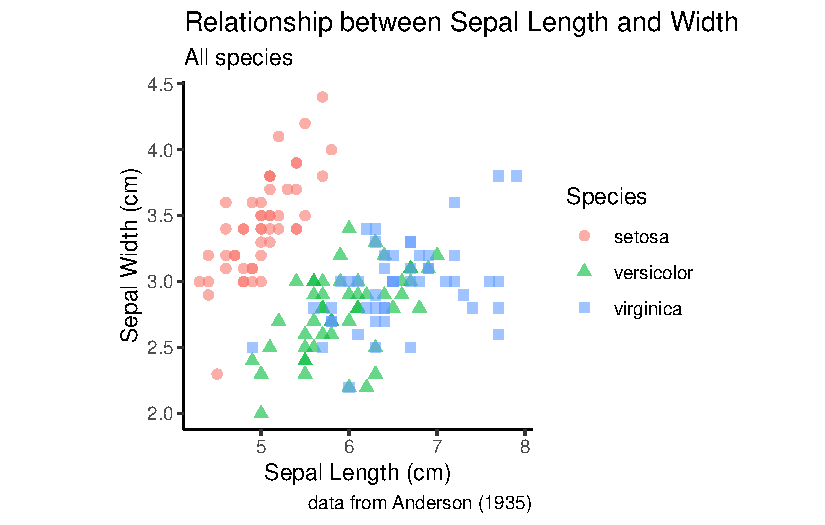
\includegraphics{Week1Lecture2_files/figure-pdf/unnamed-chunk-2-1.pdf}

}

\end{figure}

\hypertarget{why-use-r}{%
\subsection{Why use R?}\label{why-use-r}}

\begin{itemize}
\item
  R is a versatile software platform focused on data and visualization
\item
  R is free to use
\item
  \textbf{R has a large and active user base}
\end{itemize}

\hypertarget{what-we-need-from-you}{%
\subsection{What we need from you}\label{what-we-need-from-you}}

\begin{itemize}
\item
  Be respectful
\item
  Attend lectures and recitations
\item
  Submit assignments on time
\item
  If there is something you don't understand or want to know more about,
  say so
\item
  If you hear something you disagree with, say so
\end{itemize}

\hypertarget{learning-how-to-ask-questions}{%
\subsection{Learning how to ask
questions}\label{learning-how-to-ask-questions}}

``Beginners face a language problem: they can't ask questions because
they don't know what the words mean, they can't know what the words mean
until they can successfully use the system, and they can't successfully
use the system because they can't ask questions.''

-Phil Agre, \emph{How to help someone use a computer}


\includegraphics{InClassStatic/worksDoesntWork.jpg}

\hypertarget{course-assessment}{%
\subsection{Course assessment}\label{course-assessment}}

\begin{longtable}[]{@{}
  >{\raggedright\arraybackslash}p{(\columnwidth - 6\tabcolsep) * \real{0.3429}}
  >{\raggedright\arraybackslash}p{(\columnwidth - 6\tabcolsep) * \real{0.1143}}
  >{\raggedright\arraybackslash}p{(\columnwidth - 6\tabcolsep) * \real{0.2143}}
  >{\raggedright\arraybackslash}p{(\columnwidth - 6\tabcolsep) * \real{0.3286}}@{}}
\toprule\noalign{}
\begin{minipage}[b]{\linewidth}\raggedright
Assessment
\end{minipage} & \begin{minipage}[b]{\linewidth}\raggedright
Weight
\end{minipage} & \begin{minipage}[b]{\linewidth}\raggedright
Due Dates
\end{minipage} & \begin{minipage}[b]{\linewidth}\raggedright
Week Number
\end{minipage} \\
\midrule\noalign{}
\endhead
\bottomrule\noalign{}
\endlastfoot
Lab exercises & 30\% & Weekly & Weeks 1 - 12 \\
Coding assignments & 25\% & Varies & Weeks 4, 6, 8, 10, 12 \\
Visualization critique & 10\% & Varies & Starting Week 4 \\
Project proposal & 5\% & October 17th & Week 7 \\
Project notebook & 15\% & November 30th & Week 13 \\
Project poster & 15\% & December 7th & Week 14 \\
\end{longtable}

\hypertarget{resources}{%
\subsection{Resources}\label{resources}}

\begin{figure}

{\centering 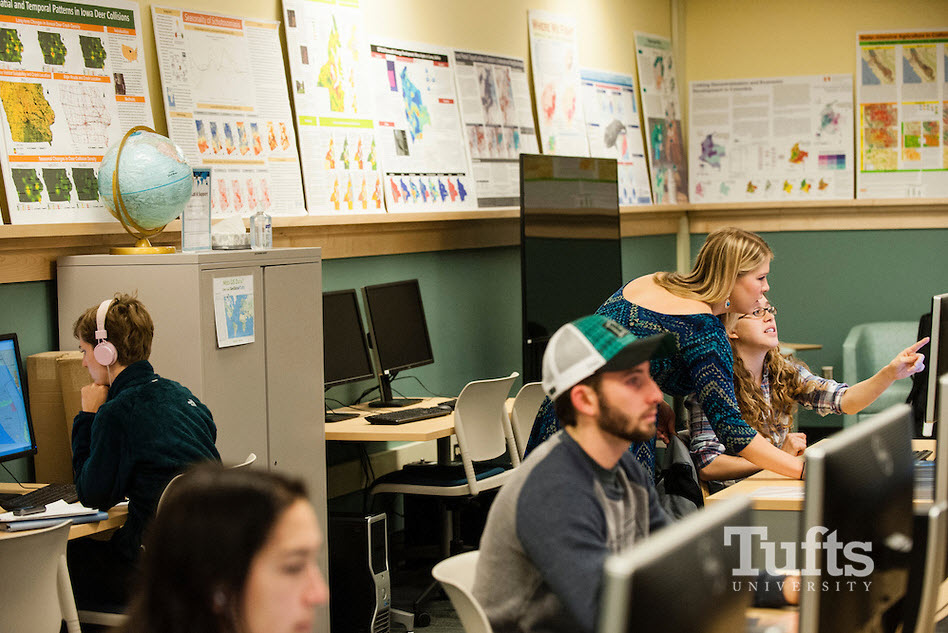
\includegraphics{Week1Lecture2_files/mediabag/Carolyn-helping-Madd.jpg}

}

\caption{Data Lab at Tufts
(https://sites.tufts.edu/datalab/services-support/student-lab-assistants/)}

\end{figure}

\hypertarget{questions}{%
\subsection{Questions?}\label{questions}}



\end{document}
